\chapter{Plan}
    
    This chapter provides information on the current state of the project at the approximate point of submission of this report. The chapter is divided into two sections:
    
    \begin{itemize}
    \item \textbf{Project Status}: Covers the current status of the project, implementation details and current AI ability.
    \item \textbf{Plan for Remainder of Project}: Covers plans for the remaining portion of thr project, classified in terms of weeks.
    \end{itemize}

    \section{Project Status}
    
    \subsection{Behavior Tree Design}
    
    For the purpose of this project, there was the necessity to develop a Behavior Tree data structure. Our implementation makes use of the \textbf{Composite Design Pattern} and the UML class diagram in Figure~\ref{img:uml_bt} shows our implementation. 

    \begin{figure}[h]                
        \begin{center}
            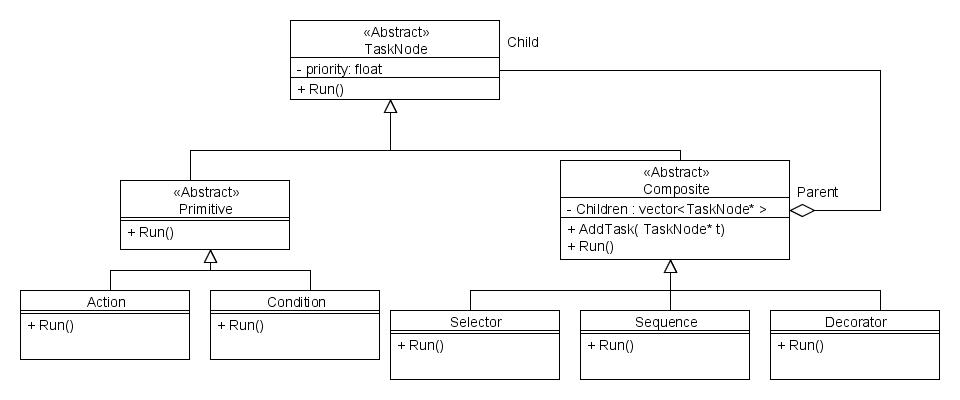
\includegraphics[scale=0.45]{images/uml_bt.jpg}
            \caption{UML Diagram for Behavior Trees}
            \label{img:uml_bt}
        \end{center}            
    \end{figure}
    
    \begin{itemize}
    \item The nodes of a Behavior Tree are of the \emph{abstract class}~\texttt{TaskNode}. 
    \item Two derived classes,~\texttt{Primitive} and~\texttt{Composite}, inherit from the~\texttt{TaskNode} class.
        \begin{itemize}
        \item Concrete classes~\texttt{Action} and~\texttt{Condition} are derived from~\texttt{Primitive}
        \item Concrete classes~\texttt{Selector},~\texttt{Sequence} and~\texttt{Decorator} are derived from~\texttt{Primitive}
        \end{itemize}   
    \end{itemize}    
    
    
    \subsection{System Design}
    
    The entire system consists of two main components - the DEFCON API and the Behavior Trees. As we can see from Figure~\ref{img:dependency}, the API's Bot class makes use of the Behavior Trees in order to execute AI logic and behavior. At the same time, the Behavior Trees need to be able to access the API calls to perform checks on the game state as well as executing commands. 
    
    \begin{figure}[h]                
        \begin{center}
        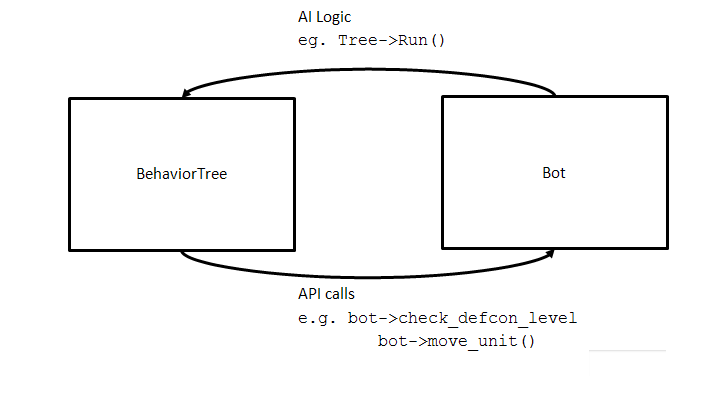
\includegraphics[scale=0.3]{images/dependency.png}
        \caption{Dependence of both the Behavior Tree and the Bot's API on each other}
        \label{img:dependency}
        \end{center}            
    \end{figure}
    
    \pagebreak
    
    Thus, in order to adhere to one of the core depency principles of having non-cyclic dependencies between classes, we have made use of the \emph{abstract client pattern}, which is illustrated by Figure~\ref{img:abstractclient}.
    
    \begin{figure}[h]                
        \begin{center}
            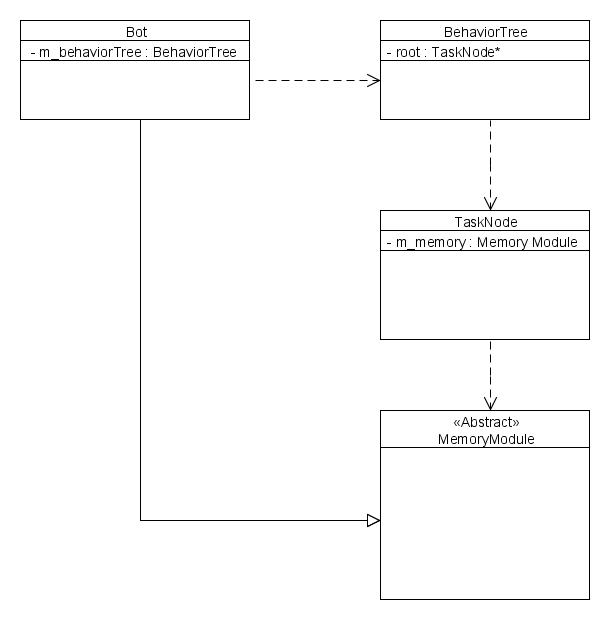
\includegraphics[scale=0.3]{images/uml_sysdesign.jpg}
            \caption{Abstract Client Pattern to prevent cyclic dependcies}
            \label{img:abstractclient}
        \end{center}            
    \end{figure}
    
    In this case, the Behavior Trees make use of what we term as a \textbf{MemoryModule} abstract class, and this essentially paves the way to to modularizing the Behavior Trees, make them reusable for any other application that may require it. For example, in the event a new game wanted to make use of the Behavior Trees, it would essentially ensure expose its API as a derived class of the MemoryModule abstract class, and create TaskNodes specific to that particular game.
    
    \newpage
    
    \subsection{AI Bot abilities} 

    At the point of writing, the AI is capable of playing the game of DEFCON, and more specifically, exhibits the following abilities:
    
    \begin{enumerate}
    \item Ability to place all 3 structure types - namely \textbf{RadarStations}, \textbf{Silos} and \textbf{AirBases}
    \item Ability to create and place fleets of any of the 3 naval forces types - \textbf{Battleships}, \textbf{Carriers} and \textbf{Submarines}
    \item Fleets are able to select a target destination and orders are sent for it to proceed to destination automatically.
    \item \textbf{Fighters} are launched to provide scouting at random locations
    \item Silos convert state to \textbf{Launch Mode} upon activation of DEFCON5, and target opponent cities.
    \end{enumerate}
    
    These abilities cover the main abilities, and allow the bot to perform actions throughout all 5 DEFCON levels. Target coordinates are now randomly picked by the bot, and in the next section we cover plans to improve upon this bot by evolving its behavior trees. 
    
    For reference, the behavior trees for each DEFCON level can be found in page~\pageref{app:defconbts} of the Appendix.
    
    \section{Upcoming Plans}
    
    The current abilities of the bot exhibits a naive players' approach to the game of DEFCON. The remainder of the project focuses heavily on improving upon this bot. More specifically, the evolving of the bots existing behavior trees, in hope of allowing the bot to gradually adapt and learn to play the game better. 
    
    A backlog of tasks pertaining to this project is included in page~\pageref{app:backlog} of the Appendix - which cover completed tasks, tasks in progress and tasks planned for the future. Here, we break down the plan into blocks of weeks, corresponding to the Department of Computing's calendar.
    
       
    \begin{center}
    \begin{tabular}{ | l | l | p{7cm}| }
    \hline
    \textbf{Term \& Week} & \textbf{Dates} & \textbf{Description} \\ \hline \hline
    Term 2 Week 06 & 15 FEB - 21 FEB & Begin evolution of Silo Placement. Submission of Interim Report. \\ \hline
    Term 2 Week 07 & 22 FEB - 28 FEB & Evolution of Silo Placement, working with Robin Baumgarten to refine API to allow collection of required data from DEFCON. Explore 2 fitness functions \\ \hline
    Term 2 Week 08 & 01 MAR - 07 MAR & Evolution of Fleet movement coordination, aim to get Fleets to identify "ideal" positions to place themselves for synchronised attack \\ \hline
      Term 2 Week 09 & 09 MAR - 14 MAR & Evolution of Aerial movement coordination. Aim to get Fighters to maximise fitness function or locating enemies, and Bombers to synchronise attacks \\ \hline
      Term 2 Week 10 & 10 MAR - 21 MAR & Coordinating evolved existing behaviors, aiming to combine abilities and provide global evolution of the AI \\ \hline
      Term 2 Week 11 & 22 MAR - 28 MAR & Collect preliminary statistics to assess current bot's abilities \\ \hline
      Easter Break & 29 MAR - 26 APR & Study break for examinations, code tweaking, refining and catch up on any implementation that was not able to be completed \\ \hline 
      Term 3 Week 01 & 26 APR - 02 MAY & Examinations \\ \hline
      Term 3 Week 02 & 03 MAY - 09 MAY & Examinations \\ \hline
      Term 3 Week 03 & 10 MAY - 16 MAY & Examinations \\ \hline
      Term 3 Week 04 & 17 MAY - 23 MAY & Assuming implementation working and performing desirably, begin work on reactive planning for fleet coordination \\ \hline
      Term 3 Week 05 & 24 MAY - 30 MAY & Work on reactive planning for Aerial coordination and movements \\ \hline
      Term 3 Week 06 & 31 MAY - 06 JUN & Consolidating report, findings and evaluation \\ \hline 
      Term 3 Week 07 & 07 JUN - 13 JUN & Consolidating report, findings and evaluation \\ \hline 
      Term 3 Week 08 & 14 JUN - 20 JUN & Final Report Submission \\ \hline
      Term 3 Week 09 & 21 JUN - 26 JUN & Presentation \\   
    \hline
    \end{tabular}
    \end{center}
    
    
      
    

